%%
%% Section 3
%%
%% 概要
%% 背景と目的
%% 方法と実現可能性
%% 期待される成果
%% 日本の独自性
%% 他のプロジェクトとの関係
%% 要求される装置とその仕様
%%
\section{日本が狙うサイエンス}\label{transients.s3}

本節では、SKAを用いた日本が主導するサイエンスについて述べる。
その中で、あるサイエンステーマを実現し成果を出すために、SKAに対してどのような装置要求をするべきか、あるいはSKAをどのように運用するべきかという戦略について言及する。
ただしSKAは既にそのデザインがおおよそ決まっているため、大幅な装置変更などは望めないことも考慮して、現状のデザインでどの程度のサイエンスが行えるか、ということについて主に述べる。

本研究は、宇宙における突発現象、変動現象を観測することによって、時間的に異なる宇宙の様相を捉え、そこから未解明の物理に迫ろうとするものであり、キャッチフレーズとして
\begin{center}
{\large \bf 「ダイナミックな宇宙を解き明かす時間領域の天文学」}
\end{center}
と題し、以下のようなサイエンスを提案する。
それらのサイエンスを日本で主導するため、SKAへ日本が参加することの重要性とSKAに対する要求に言及する。
\begin{itemize}
	\setlength{\leftskip}{3zw}
	\item [\ref{transients.s3.sn}] 系外超新星
	\item [\ref{transients.s3.snr}] 超新星残骸における粒子加速の現場、および星間物質と磁場の相互作用
	\item [\ref{transients.s3.grb}] 電波によるガンマ線バーストの即応追観測
	\item [\ref{transients.s3.magnetars}] マグネター磁気圏の解明
	\item [\ref{transients.s3.agn}] 死んだ電波銀河のシェルからの放射
	\item [\ref{transients.s3.gw}] 重力波--電波マルチメッセンジャー観測
	\item [\ref{transients.s3.frb.magnetism}] FRBの偏波の可能性と宇宙磁場	
	\item [\ref{transients.s3.unknowns}] 未知の突発天体の探査
	\item [\ref{transients.s3.requirements}] 突発天体研究のためのSKAへの要求
\end{itemize}

%%
%% Author: 前田啓一
%%
\subsection{系外超新星} \label{transients.s3.sn}

爆発直後の若い (一年程度以内の) 超新星における電波放射として支配的な機構は、超新星放出物質と星周物質の相互作用により発生する衝撃波と、そこで加速される相対論的電子からのシンクロトロン放射である \citep[e.g.,][]{1998ApJ...499..810C}。
これは現在の電波望遠鏡にとってはそれほど強い電波源ではなく、典型的な検出例では5~GHzにおいてピーク光度が$10^{27}~\text{erg}~\text{s}^{-1}~\text{Hz}^{-1}$ 程度の現象である \citep[e.g.,][]{2014arXiv1409.1827P}。
したがって、これまで電波観測されている数十例の系外超新星は、主に数十Mpc程度以内の距離で発生したものに限られており、非常にバイアスのかかった、限られたサンプルしか存在しない。

超新星の電波帯域における多様性は大きく、GRBに付随する極超新星 (SN 1998bwなど: \citealp{1998Natur.395..670G})、それと関連があると考えられている「相対論的」超新星 (SNe 2009bb, 2012ap: \citealp{2010Natur.463..513S})、あるいはIIn型超新星と呼ばれるタイプの一部 \citep[e.g.,][]{2012ApJ...755..110C} においては、その光度は$10^{29}~\text{erg}~\text{s}^{-1}~\text{Hz}^{-1}$ まで増光する。
タイムスケールも様々であり、5~GHz帯では典型的に数十日程度でピークを迎えるが、数年以上増光し続けるタイプのものも存在する。

観測されている電波放射の多様性は、超新星爆発により放出された物質の運動エネルギーおよび星周物質密度・分布の多様性を反映していると考えられ、電波放射の情報から星周物質密度などが導かれている \citep[e.g.,][]{2012ApJ...758...81M}。
一般に可視光観測からは星周物質の情報を直接導出することはできない。
超新星からの電波放射は、爆発直前の数十~数百年にわたる親星からの質量放出を反映するため、電波帯域における観測は、恒星進化論でも最大の謎の一つである大質量星の終末期の性質、超新星に至る直前の進化を知るためのユニークな手段である。
また、超新星残骸からの多波長放射により宇宙線加速機構の研究が進んでいるが、若い超新星においては衝撃波速度とダイナミクス、星周物質の密度が大きく異なる。
このため、宇宙線加速機構について超新星残骸を用いた研究とは別確度から切り込む新たな手段になると期待される。

SKAによる系外超新星研究は、主に可視で発見された超新星の即応追観測、SKA自体による電波サーベイの二つを並行して行うべきである。
現在世界中で様々な突発現象・超新星可視光サーベイが進行しており、SKAの時代には Large Synoptic Survey Telescope (LSST) の稼働が見込まれる。
日本においても木曽シュミット望遠鏡やすばる望遠鏡 Hyper Suprime-Cam (HSC) を用いた可視サーベイ計画が進展しつつある。
さらに、可視赤外大学間連携を通し可視・近赤外追観測の枠組みも整備され、恒星進化・超新星の理論研究を行うグループも多数存在しているなど、SKAの時代における即応追観測について存在感を発揮するための下地ができていると考えられる。
また、日本は歴史的に見ても電波観測におけるプレゼンスを発揮しており現在も大学間連携などを通し維持・発展しているのに加え、超新星電波放射の理論研究の下地もできつつある。
これらを総合し、可視--電波--理論を組み合わせた研究を進めるにあたり十分な下地ができていると言えるであろう。

\subsubsection{(1) 観測数の飛躍的増加によりもたらされる統計的理解}

超新星の性質の多様性を考えると、現在までの数十程度のサンプル数ではその全容を解明するためには全く不十分である。
SKAにおいては現在より少なくとも一桁良い観測精度を達成できるため、少なくとも数十倍の効率をもって、現在までの観測例とほぼ同等の質 (観測期間、S/N比など) のデータを取得できる。
たとえば年間一万個にのぼる発見が可能であるという見積もりも存在する \citep[e.g.,][]{2014arXiv1409.1827P}。
これにより、超新星の電波帯域における性質と可視光域における性質の関係が明らかになり、したがって爆発に至る進化 (電波) と超新星爆発の性質 (可視) の関係が明らかになるであろう。

\subsubsection{(2) まだ検出されていない電波放射の弱い超新星の研究}

従来の観測では、大半の超新星について電波放射は検出できていない。
つまり従来見つかっている超新星は、質量放出率の大きい系、爆発前に激しい質量放出をした系などが選択的に観測されたものであると考えられる。
また、既存の恒星進化理論では到底説明できないような、$0.1M_\odot~\text{year}^{-1}$以上の激しい質量放出が爆発直前に起こっている例も示唆されている \citep[e.g.,][]{2014ApJ...790L..16M}。
これらが特殊なのか一般的なのか明らかにするためには、より「弱い」電波放射をする超新星をとらえることが不可欠であり、これはSKAでなければ達成できない。

個々の問題についても、新たな電波放射検出が未解決問題解明のブレークスルーになり得る。
たとえば、Ia型超新星親星周辺の星周物質の有無・質量放出率は爆発に至る白色矮星の進化解明において最重要である \citep[e.g.,][]{2013FrPhy...8..116H}。
伴星が主系列星・巨星の場合 (single degenerate scenario: SD) には比較的濃い星周物質の存在が予測され、一方白色矮星二つの合体説 (double degenerate scenario: DD) からは希薄な周辺環境が予測される。
現在までの観測で、ごく近傍で発生した二つの超新星の星周密度について強い上限がついており、SD説に対し否定的な結果が得られている \citep{2014arXiv1409.1827P}。
同様の近傍Ia型超新星について弱い電波を実際に検出すること、さらに多くのサンプルについて強い上限値をつけることで、この議論に決着がつくであろう。
同様の議論はIa型超新星・重力崩壊型超新星の両方で見られる多様性の起源の解明のための大きな一歩となり得る。

\subsubsection{(3) 可視光では観測できない激しい星形成を起こしている銀河での超新星の検出と研究}

重力崩壊型超新星は大質量星の爆発であるため、その多くは激しい星形成を起こしている銀河で発生しているはずである。
しかし、luminous infrared galaxy (LIRG) や ultra luminous infrared galaxy (ULIRG)\footnote{光度が$10^{11}L_\odot$を超えるような赤外線で明るい銀河を LIRG とよび、$10^{12}L_\odot$を超えるものを ULIRG とよぶ。} といった星形成の激しい銀河は、一般的に可視光域では吸収が大きい銀河であり、そこで発生した超新星を可視光サーベイで発見することは困難である。
近年においては adaptive optics (AO) を用いた近赤外サーベイ、空間分解能の高い電波サーベイもなされているが、未だに数例の観測例が知られているだけである \citep[e.g.,][]{2007ApJ...659L...9M}。

超新星のイベントレートの測定は直接的な星形成率測定を与え、特に高赤方偏移に行くほど「隠された」星形成の割合は増えるため、イベントレートの解明は星形成史や初期質量関数の研究、超新星に至る恒星進化の研究にとって重要な要素である。
同時に、星形成の盛んな環境における超新星の性質が、これまで知られている超新星と同様であるかは自明ではない。
SKAにおける電波での広視野サーベイにより、このようなバイアスのかからない超新星のイベントレートや、様々な環境における超新星の性質・恒星進化、および初期質量関数の情報が得られるであろう。

\subsubsection{(4) 可視光観測とのシナジーによる近傍超新星の包括的研究}

これまでごく近傍の一握りの超新星について可視--電波の双方からの研究がなされているが、そのサンプル数の増大は重要である。
サンプル数が増えることによって、電波からわかる「親星の質量放出」と可視光からわかる「超新星の性質」との関係 (前述) や、様々な物理状況 (衝撃波速度、星周物質密度) における非熱的粒子加速 (後述) に加え、可視--電波観測のシナジーにより多くの新たな情報が得られる。
たとえば、電波による高い空間分解能の観測によって、ごく近傍の超新星については衝撃波伝搬の様子が直接撮像により求まる \citep[e.g.,][]{1995Sci...270.1475M}。また、爆発直後からの電波追観測により親星を衝撃波が突き抜けた直後 (ショックブレークアウト) の衝撃波速度を測定し、これから親星半径の情報を得ることができる \citep{2013ApJ...762L..24M}。
これらは最新の可視光観測手法と相補的であり、新たな研究分野を創出すると考えられる。

\subsubsection{(5) 強い衝撃波における相対論的電子加速機構、電子注入問題}

相対論的粒子加速機構は天体物理学における最重要未解明問題の一つである。
加速陽子の最大エネルギーが近年明らかになりつつあるが、それと同様に大きな問題として低エネルギー電子注入問題がある。
星周物質中を衝撃波が伝搬する若い超新星においては、物質密度したがって増幅磁場密度が大きいことがわかっており、GHz帯での観測によりMeV--GeV域の電子からの放射をとらえることができる \citep{2013ApJ...762L..24M}。
さまざまな星周物質密度をもつ異なる超新星の観測を包括的に行うことで、MeV--GeV域での加速電子スペクトルを得ることができるほか、ALMAなどによる高周波観測を組み合わせることで、個々の超新星における低エネルギー非熱的電子スペクトルを得ることができるであろう。
これは、電子注入問題を解明する上でのブレークスルーになり得る。
また、様々な環境で発生し様々な衝撃波物理状況を持つ様々な超新星を観測することにより、電子加速効率などを統計的に調べることが可能になり、これをもって粒子加速機構に必要・重要な条件を探ることができるであろう。




%%
%% Author: Shiu-Hang Lee, 長瀧重博
%%
\subsection{超新星残骸における粒子加速の現場、および星間物質と磁場の相互作用} \label{transients.s3.snr}

質量の大きな星々はその最期に超新星爆発とよばれる大爆発を起こすが、その後に何も残さない訳ではなく多様な物理現象がその後も続く。
多くの場合、超音速で膨張する星の残骸 (イジェクター) が様々な星間物質、あるいは星が「生前」放出した星風に衝突することによって衝撃波を形成する。
また衝撃波によってガスが高温に加熱され、陽子・電子などの帯電粒子が高エネルギーに加速されるなど非熱的な現象をも起こし、その結果電波・赤外線・可視光からX線・ガンマ線に至るまで多波長で見られる星雲状の天体を残す。
その何光年にも広がる天体は超新星残骸と呼ばれる。

超新星残骸は銀河の中の物理現象において様々な重要な役割を果たしていると考えられている。
例えば銀河系内宇宙線の生成、鉄など生命に不可欠な重元素の放出、星の形成、星間磁場の増幅などは、超新星残骸によって引き起こされるものである。
しかし、これまでに数多くの観測、理論モデリング、シミュレーションがなされてきたにもかかわらず、残骸中の物理は未だ完全には解明されておらず、実に複雑な天体であることが分かっている。
その問題が未解決であることの原因は、超新星残骸が年齢、親星の構造・組成、周囲の環境などの違いによって著しい多様性を示すこと、また既存の観測装置の性能限界とサンプル数の不足のためである。
そこでSKAのような、従来の観測装置の性能を遥かに超える次世代望遠鏡が、超新星残骸の理解のために非常に期待されている。
SKAを用いた科学や、そのためのSKAへの要求としては、以下のようなものが挙げられる。

\paragraph{(1) サンプル数の増大}
今まで発見された銀河系内の超新星残骸の数は僅か300に満たないが \citep{2014BASI...42...47G}、超新星の発生率を考えれば \cite[e.g.,][]{2006Natur.439...45D}、この数字は極端に少ない。
このことはつまり、まだ発見されていない超新星残骸が数多く残っているということであり、SKAの空間分解能と高感度があれば、これまでは暗すぎて観測できなかった残骸や、さらには系外天体の残骸についても多数発見出来ると考えられる。
また近傍銀河 (大マゼラン星雲、M33銀河など) の超新星残骸を探査することにより、若い残骸から古い残骸まで、超新星残骸の全体像を統計的に描けるようになる。
近傍銀河内の超新星残骸観測により、吸収のために観測しにくい天の川銀河内の残骸の真の分布も間接的に予想できるかもしれない。
更に他波長の観測装置 (Astro-H、CTA、ALMAなど) と緊密に連携し、多くの残骸を幅広いエネルギー域で調べることも可能となるだろう。

\paragraph{(2) 残骸の真の構造}
電波連続波で見る残骸はほとんどシェル状だが、その内部構造は複雑であり、特に衝撃波の周りではフィラメント状の構造が見つかる場合がある \citep[][]{1997ApJ...491..816R,2007A&A...471..537C,Reynolds2011}。
SKAを駆使することで、今まで感度不足のため見えなかった細かい構造を定量化し、モデリングを通して超新星残骸の真の三次元構造を明らかにできるだろう。
特にX線など他の波長との相関がより明確にわかるようになるため、超新星残骸中の非熱電子と磁場強度の分布を同時に解明できるようになり、無衡突衝撃波における粒子加速と磁場増幅の物理への理解を更に深めることにつながる。

\paragraph{(3) 粒子加速と磁場}
超新星残骸の電波連続波は主に加速された非熱電子によるシンクロトロン放射である。
SKAは広い波長帯をカバーしており、場所ごとの非熱電子のベキを精度よく測定できるようになると期待される。
また高感度で偏波観測を行えば、偏波率の小さい残骸に対しても、残骸内外の磁場の方向を推定することができる。
磁場の方向は衝撃波による粒子加速に大きく寄与するため \citep[][]{1996ApJ...473.1029E,2013AJ....145..104R,2014ApJ...783...91C}、SKAは高感度な偏波観測を行えるようデザインされなければならない。

\paragraph{(4) 星間物質との相互作用}
超新星残骸の多くは周りの星間物質 (星風、HI・分子雲など) と相互に強い影響を与え合い、明るい電波を放つ \citep{2000ApJ...538..203B,2012ApJ...746...82F}。
例えば、最近フェルミ衛星 \citep[e.g.,][]{2013Sci...339..807A} の観測によって、ガンマ線で明るくかつ爆発から1万年程度経った古い残骸は、そのほとんどが分子雲とぶつかっており、電波でも明るく観測されることがわかっている。
その放射機構・粒子加速機構はまだ謎のままだが、SKAによってこのような残骸を精度よくイメージングし、他の波長の観測データと組み合わせ、更にセルフコンシステントな理論モデル \cite[e.g.,][]{0004-637X-750-2-156} で解釈することにより、この謎は解明されると考えられる。
このとき他波長データとの比較のため、SKAはその資源を\Secref{transients.s2.wilkinson}で述べたVirtual Observatoryにささげることが重要である。



%%
%% Author: 長瀧 重博
%%
\subsection{電波によるガンマ線バーストの即応追観測} \label{transients.s3.grb}
宇宙最大の爆発とされるガンマ線バースト (gamma-ray burst; GRB) はまず数100~keV程度のソフトガンマ線で明るく輝き (1--10秒程度続く即時放射と呼ばれる)、次いでX線、紫外・可視・赤外光、電波など多波長で輝く「残光」と呼ばれるフェーズに移行していく。
現在GRB検出の主力観測機器はNASAのSwift衛星であり、ソフトガンマ線検出器に加えX線検出器、紫外・可視光検出器を搭載している。
視野についてはソフトガンマ線検出器が優れているのに対し、位置決定精度についてはX線検出器、紫外・可視光検出器が優れている。
従って即時放射をまず広い視野を持つソフトガンマ線検出器で同定し、直ちにその視野内をX線、紫外・可視光検出器でフォローアップすることで残光を検出、GRBの正確な位置情報を地上望遠鏡等に速報するシステムが構築されている (\Secref{transients.s1.grb})。
このシステムにより、Swift衛星によって秒角程度に絞られた位置情報を基に、すばる等の地上望遠鏡は深いフォローアップを行い、詳細な残光観測・ホスト銀河観測等を行うことが現在可能となっている。

\subsubsection{SKAへの期待と要求}
SKAの時代にSwift衛星自体が運用されているかどうかは定かではないが、類似のGRB衛星計画にはSVOM計画 (中国--フランス: \citealt{2011CRPhy..12..298P})、HiZ-GUNDAM計画 (日本: \citealt{2014SPIE.9144E..2SY}) などがあり同様の速報体制は維持されているものと考えられる。
従ってGRBはトランジェントな現象であるが、SKA自体がサーベイする必要性はそれ程高くない。
むしろ速報を受けた際に素早くフォローアップする用意をSKAは行っておくべきである。
またこれまでに観測されているGRBの典型的な電波残光のスペクトルから、GRB電波残光はGHz以上の周波数帯で明るいことが知られている。
以上の状況から、SKAによるGRB観測はたとえ視野が狭くても大きな問題ではなく、GHz以上の観測波長帯で感度の高い\skamid{}が有効であると考えられる \citep{2015arXiv150104629B}。

\skamid{}の感度を考慮すると、およそ年間数百のGRB電波残光が検出できると予想される。
この数は1997年に初めて残光が検出されて以降、観測された電波残光の総数とほぼ同程度であり \citep{2012ApJ...746..156C}、SKAは電波残光の観測例を飛躍的に増大させると期待できる。
またこれまでの統計では、発見されたGRBの約1/3の割合のみで電波残光が検出されているが \citep{2012ApJ...746..156C}、SKAによる深い観測によって``弱い''電波残光が検出されることも期待され、GRB残光の物理状況の理解がより進むと期待される。
また比較的近傍の電波残光については放射領域の固有運動の検出が期待でき \citep{2004ApJ...609L...1T}、GRBのダイナミクスに重要な情報を与えると期待できる。
遠方の電波残光については特に初期のフェーズにおいてシンチレーションによる光度変動が予想され \citep{1997Natur.389..261F}、GRBジェットの口径に強い制限を与えることもできる。
更にGRBジェットが地球を向いていない場合にも、後期にはジェットの減速に伴い口径が広がり、ついには地球で残光が検出されるという親なしGRB残光 (orphan afterglow, \Secref{transients.s1.grb}) の初検出も\skasur{}において期待できる \citep{2015arXiv150104629B}。
また起源のわかっていない short GRBの電波残光は現在まで30例強発見されているのみで、統計的に充分でない。
しかしこの限られたサンプルの中では long GRBに比べて一桁、あるいはそれ以上電波残光の強度が低い傾向が見られるという報告もある \citep{2012ApJ...746..156C}。
SKAによる高感度観測により、short GRB電波残光の特性がより明確に理解でき、short GRBの正体に迫る手掛かりにもなると期待される。

\subsubsection{日本の独自性とまとめ}
以上のようにSKAのGRBに対する科学的貢献は期待が非常に高い。
そしてSKAがその期待に応えるためには、GRBの発見速報を受けた際に、素早くそれをフォローアップできるような運用体制を\skamid{1}に課さなければならない。
また日本 (SKA-Japan) においては、日本のGRBミッション・HiZ-GUNDAMとの連携で大きな特色を打ち出すことが期待できる。
HiZ-GUNDAMは高赤方偏移 (high-z) した遠方GRBの検出を主眼においており、宇宙再イオン化期の宇宙の物理状況を解き明かすことにも貢献できるミッションである。
すなわちSKAの21~cm線観測による宇宙再電離期観測とは別のアプローチとして、SKAとHiZ-GUNDAMとの連携による{\bf 「遠方GRB・宇宙再電離期の物理状況の理解」}という日本発のサイエンスが期待でき、その意義は非常に高い。



%% Author: 榎戸 輝揚
\subsection{マグネター磁気圏の解明} \label{transients.s3.magnetars}
X線パルサーの中には、自転周期 2--12~s という遅い自転と、その自転周期が毎秒 $10^{-12}$--$10^{-10}~\text{s}$で遅くなるという極めて早い減速率を示し、そこから推定される磁場の強さが $10^{14}$--$10^{15}~\text{G}$ にも達するものが報告されている \citep{2008A&ARv..15..225M}。
さらに、観測されるX線光度が中性子星の自転では説明できないこともあり、それらのパルサーは内部に蓄えた磁場を解放して輝く超強磁場の天体と考えられるようになり、マグネターと呼ばれるようになった \citep{1995MNRAS.275..255T}。
このマグネターは、これまで銀河系内に 2000 個以上見つかってきた通常の回転駆動型パルサーとは異なる種族として、超新星爆発の機構や磁場の起源、強磁場の物理などの観点からも注目を集めている。

Swift衛星によって、突発的にX線で増光する銀河系内のマグネターも数多く見つかるようになり、すでに 30 個程度が知られている。
この発見をもたらした X 線アウトバースト現象では、$k_\text{B}T \sim 0.3~\text{keV}$ にピークをもつ星表面の熱的放射が増光するとともに、硬X線にピークをもつショートバーストを頻発し 100~keV 近くに向かって伸びる硬X線のべき放射も検出されるようになってきた \citep{2010ApJ...715..665E}。
こういった突発現象は通常の電波パルサーと異なるマグネターの特徴で、多波長でのフォローアップが急速に進展している。

通常の電波パルサーと異なり、定常的に明るく輝くマグネターでは、多くの場合電波のパルス放射が検出されていない。
たとえばGreen Bank 望遠鏡を用いた 1950~MHzの電波観測では、マグネター候補7天体で電波パルスは観測されなかった \citep{2012ApJ...744...97L}。
しかし一方で、X線アウトバーストを生じた際には電波が放射されるという例が報告されるようになってきた。
2003年に発見された XTE~J1810-197 \citep{2006Natur.442..892C} や2007年に突発増光した 1E~1547.0-5408 (PSR~J1550-5418; \citealt{2008ApJ...679..681C}) では、GHz 帯域でフラットなスペクトルを示し、100\% に近い直線偏光を示すなど、共通点をもった電波パルスが報告された。
さらに、電波観測によって最初に発見されたマグネター PSR~J1622-4950 \citep{2010ApJ...721L..33L}や、2013 年に銀河中心で見つかったマグネター SGR~1745-29 (PSR~J1745-2900; \citealt{2013ApJ...770L..23M}, \citealt{2014ApJ...780L...3S}) など、電波帯域でもマグネターの観測例が蓄積されつつある。

マグネターはX 線で卓越した放射を示すため、これまでは主に高エネルギー帯域の観測が主だったが、トランジェント型のマグネターの電波観測が新しい観測の窓とし
て開かれつつある。
また、定常的に明るい天体からも微弱な電波パルスが検出できるようになることも期待される。
従来、電波パルサーの多波長に渡るパルス研究がパルサー磁気圏の理解を進ませたように、SKA による電波観測を可視光やX線と組み合わせた多波長の突発現象観測が、マグネターの磁気圏の解明の伴になると期待できる。
%%
%% Author: 伊藤裕貴
%%
\subsection{死んだ電波銀河のシェルからの放射}\label{transients.s3.agn}
電波銀河の主な放射源は、AGNジェットによって形成される電波ローブと呼ばれる広がった構造である。
観測されている電波銀河のサイズは幅広く分布しており、kpc未満のものからMpcを超えるようなものまで存在している。
電波銀河の大きさは、主に年齢 (ジェットの中心核からの噴出が維持されている時間) によって決まり、小さいものは若く、大きいものは年老いていると考えられている。
したがって、小さい電波銀河はいずれ大きい電波銀河に成長するといった描像が広く受け入れられている。

しかしながら、単純に全ての電波銀河が10~kpcを超えるような大きさに成長できるのかはよく分かっていない。
というのも、理論的には 10~kpcに満たない小さくて若い電波銀河 (年齢$10^3$--$10^5$歳の電波銀河) の割合は全体の約 0.01\% と予測されるが、実際の観測では全体の約 10--30\% を占めており、年老いた銀河が予測より少ないためである \citep{Orienti01032010,2010MNRAS.408.2261K}。
この未解決問題について様々なシナリオが提唱されてきているが、一つの自然な解釈は、大多数の電波銀河が若い段階でジェット活動を停止もしくは休止し、成長が止まってしまい「死んでいる」とする解釈である。

このシナリオを検証するためには、死んだ電波銀河を観測でとらえる必要性があるが、ジェットの活動性を失った電波ローブは急激に暗くなってしまうため、従来の観測施設でとらえる事は困難であり、現状は候補天体が数例見つかっている程度である。
さらに最近の理論研究からは、ローブは暗くなるだけではなく放射帯域が10~MHz以下となってしまうため、SKA をもってしても、死んだ天体の電波ローブからの放射を検出する事は難しい事が示されている (Ito et al., 2015, submitted to ApJ)。
しかし電波ローブではなく、それを取り囲む周辺物質から構成される「シェル」は、ジェットの活動が休止した後も急激には減光しないため、SKAによってとらえられる事が期待できる (\Figref{fig:transients.s3.agn.fig1})。
したがって、電波銀河の進化トラック解明への道を切り開くためには、SKAを用いてシェルの観測を行うことが不可欠である。
さらにSKAによって、AGNジェットが周辺環境に与える影響 (AGNフィードバック) や、ジェットが駆動される条件などのサイエンスに関しても迫る事が期待される。
\begin{figure}
		\centering
		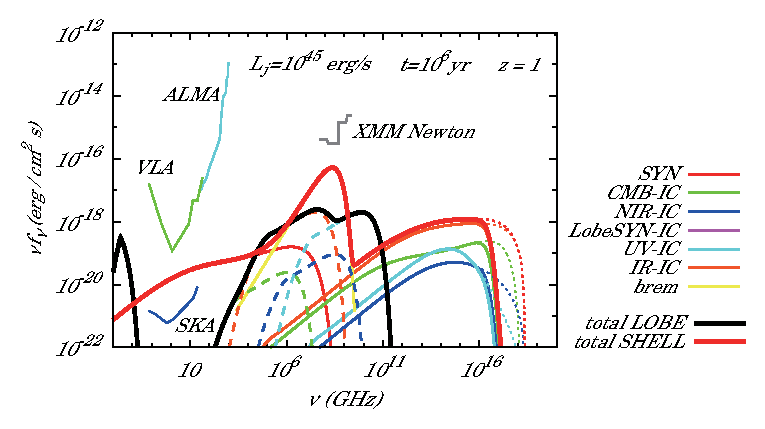
\includegraphics[width=0.8\textwidth]{transients/transients.s3.agn.fig1.eps}
		\caption{ジェットの放出が停止した (死んだ) 電波銀河に付随するローブ (黒実線) 及びシェル (赤実線) のスペクトル。
		電波銀河の年齢を$10^6$年、ジェットが活動を停止するまでの継続時間を$10^5$年と仮定し、また赤方偏移を$z=1$としている (Ito et al., 2015, submitted to ApJ)。}
		\label{fig:transients.s3.agn.fig1}
\end{figure}%

%% Author: 端山和大

\subsection{重力波--電波マルチメッセンジャー観測} \label{transients.s3.gw}
近年、オーストラリアのParkes電波望遠鏡によりFRBと呼ばれる継続時間数msの突発的な電波天体が相次いで観測され (\Secref{transients.s1.frb})、日本でも \Figref{fig:transients.s3.gw.nasu}の那須電波観測所によって、数分から数日といったFRBより長いタイムスケールの突発天体 (WJN電波トランジェント; \Secref{transients.s3.unknowns}) が観測されている。
こういった電波帯域における突発天体は未だ対応天体が発見されておらず、その起源の解明はこれからの電波天文学にとって重要なテーマの一つである。
\begin{figure}
	\centering
	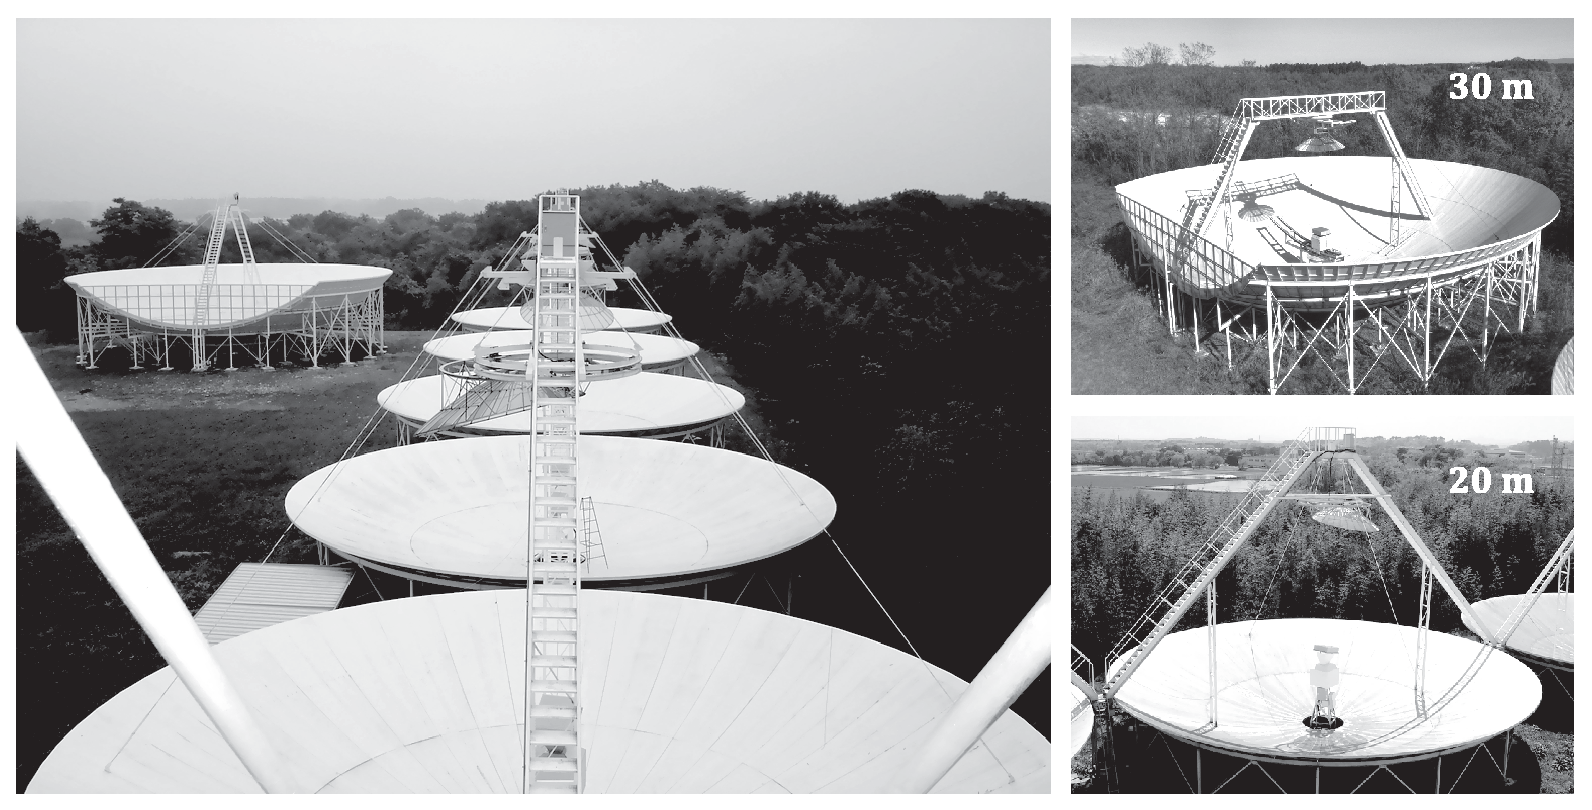
\includegraphics[width=1\textwidth]{transients/transients.s3.gw.nasu.eps}
	\caption{那須電波観測所。口径 20~m の電波望遠鏡8基、30~mの電波望遠鏡1基をもつ。}
	\label{fig:transients.s3.gw.nasu}
\end{figure}%

こうした突発天体は、そのエネルギーとタイムスケールから、重力波を伴うような天体爆発現象である可能性が示唆されている。
FRBのモデルとしては、重力波天体として最有力候補の一つである中性子連星合体時に起きるシンクロトロン放射\citep{2013PASJ...65L..12T}があり、またWJNイベントのモデルとしては、中性子星連星合体後に起きる電波アフターグローモデルが考えられる \citep{2011Natur.478...82N}。
さらに連星合体の際は、\Secref{transients.s1.grb}で述べたようにshort GRBも付随することが予想される。
そこで重力波と電波を中心とした、「マルチメッセンジャー観測」と呼ばれる多粒子・多波長による連携観測により、天体現象の多角的理解を目指す観測体制の構築が重要になる \citep{2012IAUS..285..331H}。

FRBの本来のイベントレートはおよそ$2 \times 10^4~\text{Gpc}^{-3}~\text{yr}^{-1}$ と見積もられており、現在建設中の重力波望遠鏡が見通せる、地球から$200~\text{Mpc}$ 以内で起こりうるFRBは、年間$160$ 個程度と考えられる。
このイベントレートは現在見積もられている連星中性子星合体のイベントレートの誤差範囲内にある。
もしFRBの起源が重力波天体であり、かつすべて検出できるならば、2020年には年間$160$程度の重力波--FRB同時観測が行われ、統計的な議論もできるようになると考えられる。
こうした突発天体を捉えるためには広い視野で長期間観測して天球上を走査することが最も有効になる。
SKAで採用が検討されている Phased Array Feed (PAF) は $18~\text{deg}^2$ という広い視野を持ち、\skasur{1} プログラムでは1年間で$550$時間、走査領域にして$10,000~\text{deg}^2$をカバーすることが予定されており、非常に有望な重力波マルチメッセンジャー観測体制を担う望遠鏡である。
さらにSKAでAdvanced Instrumentation Program (AIP) となっているMid-frequency Aperture Array (MAA) は、$200~\sqdeg$という驚異的な広視野を持ち、その実装は電波天文学のみならず重力波天文学にとっても極めて重要である。

\subsection{FRBの偏波の可能性と宇宙磁場} \label{transients.s3.frb.magnetism}

今現在までに、FRBに有意な直線偏波は検出されていない\footnote{円偏波は1例観測された \citep{2015MNRAS.447..246P}。}。それがFRB現象に普遍的な現象なのか、または偶然なのか、その判断をするにはまだ発見数はあまりにも少ない。もしFRBに直線偏波が含まれるなら、ファラデー効果の分散測度 (DM) に加えてファラデー回転測度 (RM) も計測できる可能性がある。そうなった場合、密度重みつき視線平均磁場強度$\langle B_\parallel \rangle $をDMとRMの定義から
\begin{equation}
\langle B_\parallel \rangle =\frac{{\it RM}}{{\it DM}}
\end{equation}
という式で簡単に求めることができる。FRBが系外起源であるならば、この磁場強度の推定には銀河間磁場の情報を含む。電波銀河など系外偏波源を使ってRMを測る場合はDMは測らない (測れない) ため、このように単一観測から磁場強度まで推定できるのは画期的なことである。一つの視線だけでは系内と系外の寄与を切り分けるのは難しいかもしれないが、沢山の観測で統計を高めることで、銀経・銀緯に依存しないが赤方偏移に依存するような「超過成分」として銀河間磁場の寄与が議論できるかもしれない。SKAのサーベイ能力は、そのような統計的な議論をはじめて可能にするだろう。具体的で確実な調査の方法論を理論的に検討していくことも不可欠であるが、日本は銀河間磁場の調査で世界をリードしているので\citep{2014PASJ...66...65A,2014ApJ...790..123A}、日本のSKAサイエンスの特色の一つとできるだろう。FRBが銀河間磁場を探る新しい方法となるかもしれない。
%% Author: 青木貴弘
\subsection{未知の突発天体の探査} \label{transients.s3.unknowns}
{ %% Localize settings
\newcommand{\suffix}[2]{^{> #1 \, \text{mJy}} _{#2 \, \text{GHz}}}
\newcommand{\ntt}{那須 20~m 電波望遠鏡}
\newcommand{\WJN}{WJN J1443+3439}
\newcommand{\FDR}{{\it FDR}}
\newcommand{\siglevel}{\mbox{$10^{-5}$}~}
\newcommand{\ssd}{天球面密度}

%% Body
%%
%% ss1
%%
\subsubsection{従来の探査結果}
他の波長域で対応天体が見つからないような、未知の突発天体の探査が何度か行われてきている。
例えば\citet{2002ApJ...576..923L}は orphan GRB afterglow をカタログ比較によって探査し、9つの候補天体を発見した。
その後、追観測やデータの再解析によって8つが偽陽性検出であることが判明し、1つについては電波のみを放射しているII型超新星とわかりVLA~121550.2+130654 と命名された \citep{2006ApJ...639..331G,2010ApJ...711..517O}。

それ以降、未知の突発天体探査が活発化し、それらの探査結果を図示したものが\Figref{fig:transients.s3.unknowns.rate}である。
図中の各プロットは脚注に示す文献に基づいている\footnote{
\Figref{fig:transients.s3.unknowns.rate}の各プロットは次の文献をもとにしている: \citealt{2007ApJ...666..346B} (Bow07 2-month/single), \citealt{2010ApJ...725.1792B} (Bow10a/b), \citealt{2011ApJ...740...65O} (Ofe11), \citealt{2012AJ....143...96J} (Jae12), \citealt{2006ApJ...639..331G} (Gal06), \citealt{2011MNRAS.412..634B} (Ban11), \citealt{2010ApJ...719...45C} (Cro10),  \citealt{2011ApJ...728L..14B} (Bow11a/b), \citealt{2014ApJ...781...10A} (Aok14), \citealt{2010AJ....140.1995L} (Laz10)。
いくつかのプロットは\citet{2011MNRAS.415....2B}, \citet{2012ApJ...747...70F}にまとめられている。
}。
\Figref{fig:transients.s3.unknowns.rate}の横軸は観測感度、つまり最小検出フラックス密度$S$を表し、縦軸は天球上の単位面積を観測したときに、フラックス密度が$S$を超える未知天体を発見できる個数、つまり天球面上の個数密度$\varSigma (>S)$を表す。
この天球面上の個数密度 (sky-surface density) はスナップショットレート (snapshot rate) とも呼ばれ、イメージング観測の結果として導くことができる発見確率の指標であり、この量をイベントレートに換算することができる。
\begin{figure}
	\centering
	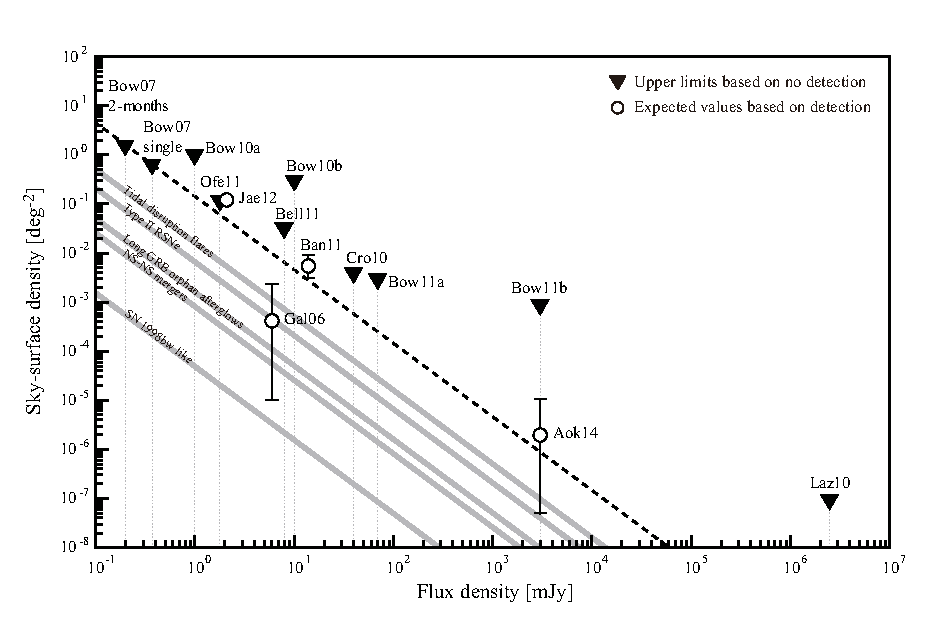
\includegraphics[width=1\textwidth]{transients/transients.s3.unknowns.rate.eps}
	\caption{未知の突発天体に対する、天球面上の個数密度$\varSigma (>S)$ とフラックス密度 $S$ の関係 \citep{2014ApJ...781...10A}。
	ただし観測周波数は考慮していない。
	三角形のプロットは突発天体が発見されなかった探査結果を示し、円形のプロットはいくつかの発見があった探査結果を示す。
	灰色の太線は\citet{2012ApJ...747...70F}によって推定された、既知天体の個数密度を表している。}
	\label{fig:transients.s3.unknowns.rate}
\end{figure}%

これらの探査によって、いくつかの候補天体が発見されてきているが、その起源のみならず発見の真偽についても確証は得られていない。
この検証のためには、従来の観測装置の性能では多くの観測時間が必要となり現実的ではなく、SKAによる広視野・高感度な探査観測が必要となる。
そこで、これらの検証のためにSKAに必要な性能を、早稲田大学の那須電波観測所による探査結果を例にして提案する。

%%
%% ss2
%%
\subsubsection{従来の探査結果の検証}
\paragraph{検証の方法}
\Figref{fig:transients.s3.unknowns.rate}の Aok14 というプロットは、那須電波観測所 (\Figref{fig:transients.s3.gw.nasu}) で行った突発天体の探査結果を示している。
その探査では、1日程度の継続時間をもつ起源不明の突発天体を発見し、\WJN と命名した \citep{2007ApJ...657L..37N}。
この発見から、周波数1.42 GHzにおいてフラックス密度3000~mJy以上を持つ未知の突発天体の個数密度は、$\varSigma \suffix{3000}{1.42} = 2^{+9}_{-1.9} \times 10^{-6}~\persqdeg$ と見積もられる\footnote{
\citet{2010ApJ...711..517O}の定義に従えばイベントレート $\mathfrak{R}$ は個数密度$\varSigma$と光度変動の継続時間$W$を用いて$\mathfrak{R} = \varSigma / W$で与えられ、那須電波観測所で発見されたWJNイベントに対しては$%
	\mathfrak{R}\suffix{3000}{1.42} = 7^{+33}_{-7} \times 10^{-4}(W/\text{day})^{-1} \persqdeg \peryr 
	= 30^{+136}_{-28} (W/\text{day})^{-1} \persky \peryr%
$
を得る。
単位 sky は全天$4\pi~\text{sr}$として定義した。
}。
したがって任意のフラックス密度$S$における個数密度は
\begin{equation}
	\varSigma^{>S}_{\text{1.42~GHz}} = 0.3~\persqdeg \times \left(  S/\text{mJy} \right)^{-3/2}
	\label{eq:transients.s3.unknowns.nasu-dens}
\end{equation}
で推定できる。
この観測結果の正当性は、広い面積を高い感度で探査することによって検証が可能である。
\Eqref{eq:transients.s3.unknowns.nasu-dens}という結果を検証するために必要な、探査観測の感度$S$と掃天面積$\varOmega$の関係は、統計的な議論によって\footnote{
突発現象の生起個数はポアソン過程であるから事象の生起間隔 $\varOmega$ は指数分布となり、突発天体を発見できる確率は$P(\varOmega)=1-\e^{-\varSigma \varOmega}$で与えられる。
このとき95\% 以上の確率で少なくとも一つの天体を発見するために必要な掃天面積$\varOmega$ は$P(\varOmega) \leq 95\%$で与えられる。
}
\begin{equation}
	\varOmega / \sqdeg > 10 \times \left( S/\text{mJy} \right)^{+3/2}
	\label{eq:transients.s3.unknowns.survey-config}
\end{equation}
で与えられる \citep{2014ApJ...781...10A}。
この関係を満たす観測を行えば95\% の確率で同様の突発天体を検出できるはずであり、もし検出できなければ\Eqref{eq:transients.s3.unknowns.nasu-dens}という観測結果は棄却されうることになる。
このようにして那須電波観測所による探査結果のみならず、\Figref{fig:transients.s3.unknowns.rate}に示す従来の結果の多くを検証することができる。

\paragraph{検証のためのSKAへの要求}
SKA Phase 1 を用いて\Eqref{eq:transients.s3.unknowns.survey-config}を満たす観測を行えば、従来の探査結果を検証することができる。
%装置要求をするにあたり、既にデザインされている性能パラメーターのいくつかを固定し、アンテナ台数と受信機冷却に関係するパラメーター、実効開口面積$A_\text{e}$とシステム雑音温度$T_\text{sys}$を不定として、感度パラメーター$A_\text{e}/T_\text{sys}$に対する要求を述べる。
GHz帯域で行われてきた従来の探査を検証するという観点からは、必要になるのは\skamid{} または \skasur{} のアンテナであり、突発天体探査で最も重要な要素は視野の広さであるから、\skasur{}が最も適したアンテナといえる。
そこで主に\skasur{1}アンテナの基本デザインをもとに、検証に必要な system equivalent flux density (SEFD) を考える。

\skasur{1} アンテナには phased array feed (PAF) とよばれるフィードが搭載される予定であり、既存のASKAPの周波数帯域を考えると、SKA1で最初に実装するのは PAF Band~2 (周波数650--1670~MHz、視野 $18~\sqdeg$) が妥当だろう。
また観測可能な帯域幅は片偏波あたり最大500~MHzとされている。
最小検出フラックスを$S_\text{min}=\text{SEFD}_\text{array}/(\eta_\text{s}\sqrt{\varDelta \nu \ \tau})$とし検出閾値を$S=7S_\text{min}$とすると、\Eqref{eq:transients.s3.unknowns.survey-config}を満たすようなSEFDは
\begin{align}
	\text{SEFD}_\text{array} 
	< 260~\text{Jy} \times \left( \frac{\varOmega}{18~\sqdeg} \right)^{2/3}
		\cdot \frac{\eta_\text{s}}{0.9} \cdot 
		\sqrt{\frac{\varDelta \nu}{500~\text{MHz}} \cdot \frac{\tau}{1~\text{hour}}}
	%&= 15~\text{Jy} \cdot \left( \frac{\varOmega}{18~\sqdeg} \right)^{2/3}
	%	\cdot \frac{\eta_\text{s}}{0.9} \cdot 
	%	\sqrt{\frac{\varDelta \nu}{100~\text{MHz}} \cdot \frac{\tau}{1~\text{min}}}
		\label{eq:transients.s3.unknowns.sefd}
\end{align}
となる\footnote{\Eqref{eq:transients.s3.unknowns.sefd}は\skasur{1}の性能を単位としているが、当然\skamid{1}への要求検討にも使用できる。}。
ここで$\eta_\text{s}$はシステム効率、$\varDelta \nu$は観測帯域幅、$\tau$は積分時間を表す。
SKAの基本的な性能はおおよそ固まっているため、例えば建設するべきアンテナの台数に着目すると、現状の単一鏡のデザイン $\text{SEFD}_\text{dish}=586~\text{Jy}$ が実現するとすれば、上記の検証観測をするには{\ 感度のみの観点からは}3台で事足りる\footnote{$\text{SEFD}_\text{array} \simeq \text{SEFD}_\text{dish}/m$, $m=\text{アンテナの台数}$。}。
ただしもちろんこの見積もりは、光度変動のタイムスケールが1時間以上の突発天体に対するものである。

\WJN の継続時間は4分以上3日以内としか制限されておらず、またGCRT J1745-3009 のように数分スケールの電波変動を起こす天体を観測しようとすると (\Secref{transients.s1.unknowns})、上記の見積もりではその観測は実現できない。
また500~MHzという帯域幅は使用可能な上限値であり、実際の観測ではより狭帯域に制限されることもありうる。
そのような状況を考え、帯域幅100~MHzを積分時間1~minで観測することを考えると$\text{SEFD}_\text{array}=15~\text{Jy}$が必要になり、その場合アンテナは40台必要になる。
ただし\skasur{1} の計画では60台のアンテナを建設予定であり\footnote{\skasur{1}アンテナ60台、ASKAPアンテナ36台で計96台のアンテナを運用することも計画されているが、本節の見積もりにASKAPアンテナは含めていない。}、$\text{SEFD}_\text{array}=10~\text{Jy}$を得られるから、上記の検証観測は十分に実施可能である。
積分時間が1~minという観測では$u$--$v$平面の埋まりが悪いが、\Figref{fig:transients.phasespace}の中央付近の空白領域を埋めることにつながり、未知の突発天体の探査には重要な時間分解能である。

\subsubsection{未知の探査}

%既に理論的に存在することは知られているが実際に観測されたことはない、あるいは数例の観測例はあるものの確証が得られていない天体、つまり\Secref{transients.s2.wilkinson}で述べた「既知の未知 (known unknowns)」の探査をすることが、今後の電波天文学にとって重要である。
%この点について、SKAは他の電波望遠鏡に比べて極めて強いアドバンテージを持っており、その探査をすることは宇宙科学にブレイクスルーを起こせる数少ない手段の一つである。

未知の天体の例としては、\Secref{transients.s1}や\Figref{fig:transients.s3.unknowns.rate}にも示した潮汐崩壊現象や orphan GRB afterglow などがあり、前者は Swift J1644+57 という観測例があるが詳細はわかっておらず、後者は観測例もない。
これらを能動的に探査することがSKAには求められ、実際に発見するために必要な性能をSKAに持たせなければならない。
そこでここでは、\skasur{1}による探査と発見のための要求性能を考える。


\citet{2012ApJ...747...70F}の見積もりによれば\Figref{fig:transients.s3.unknowns.rate}の斜線に示したように、可視光放射がないII型電波超新星 \citep{2006ApJ...639..331G} の個数密度は$\varSigma^{>S} = 6.6\times 10^{-3}~\persqdeg \times (S/\text{mJy})^{-3/2}$である。
このレートを単位にして、電波帯域における突発天体を95\% 以上の確率で発見するために必要な観測は、
\begin{align}
	\biggl( \frac{\text{SEFD}_\text{array}}{10~\text{Jy}} \biggr)^{-2}
	\biggl( \frac{\varOmega}{18~\sqdeg} \biggr)^{4/3} 
	\biggl( \frac{\eta_\text{s}}{0.9} \biggr)^2 \cdot 
	\frac{\varDelta \nu}{500~\text{MHz}} \cdot \frac{\tau}{6~\text{hour}}
	> 0.041
	\label{eq:transients.s3.unknowns.SNII}
\end{align}
という関係を満たすような観測設定をする必要がある\footnote{$\text{SEFD}_\text{dish} = 586~\text{Jy}$のSKAアンテナ60台で干渉計を構成すると、$\text{SEFD}_\text{array} = 10~\text{Jy}$を得る。}。
したがって、例えば15分程度の観測をするだけで、従来数々の電波望遠鏡を駆使してようやく発見した、可視光対応天体のないII型超新星を95\% の確率で発見できるということである。

しかし一方で、Ic型極超新星SN 1998bw (GRB 980425) と同様の突発天体を探査しようとすると、個数密度が$\varSigma^{>S} = 4.9\times 10^{-5}~\persqdeg \times (S/\text{mJy})^{-3/2}$でありイベントレートが低すぎるため、電波帯域だけで探査しようとすると約180時間の観測時間が必要となる。
これを実現するには、約1か月間に渡って受信機性能を安定化させ、かつデータ較正をするシステムが必要になるだろう。

\subsubsection{まとめ}

従来さまざまな電波望遠鏡を用いて、未知の突発天体が探査されてきているが、視野の広さと感度の高さが両立した観測は難しく、効果的な探査は行われてこなかった。
SKAはこの現状を打破し、とりわけ\skasur{} は広い視野、高い感度、高い空間分解能を同時に実現し、突発天体研究にとって強力なツールとなるだろう。
単に従来の探査結果を検証するだけならば、\skasur{1} アンテナの台数は5台もあれば可能だが、それでは理論的に予測されているが実観測例のない orphan GRB afterglow や Ia 型超新星の研究を行うことができない。
したがって現状のデザインを実現することが重要である。
そしてその探査が実現すれば、まだ観測例のない突発天体も容易に発見できると見積もられる。




} %% End of localization

%%
\subsection{突発天体研究のためのSKAへの要求} \label{transients.s3.requirements}
%%

SKAは既にデザインがおおよそ決まっており、その装置性能や運用体制に対して修正を要求することは難しい。
そのことを踏まえて本節では、現状のデザインでどの程度のサイエンスを進められるか、あるいは最低限必要な性能は何かという点について主に言及してきた。
ここではそれらについて再度簡単にまとめる。

\subsubsection{アンテナの選択}
突発天体研究の進め方は二通りあり、(1) 他波長で発見された突発天体を追観測するという方法と、(2) 新たな突発天体を求めて主体的に探査するという方法がある。
どちらの方法も重要であり、(1) では従来の望遠鏡ではなしえない感度によって、起源天体の物理の解明をめざし、(2) では、理論予測はされていてもまだ観測されていないような天体を発見し、さらには人類がまだ予想すらしていないような未知の発見を生む可能性が高い。
そして強いて言うならば、(1) は主に\skamid{}によって実施され、(2) は\skasur{}によって実施される。
また\skalow{}は装置の特色上 (1) と (2) 両方に注力できる。

\skamidsur{} はどちらも主鏡は同じものを使用するが、そのフィードや受信機系は異なり、\skamid{}は広帯域、高感度、高分解能に、\skasur{}は広い視野による探査速度に長けている。
日本の既存望遠鏡との連携という観点からは、時差のほとんどないオーストラリアに建設される\skasur{}が突発天体探査と追観測には有利といえる\footnote{ただし北半球の日本と南半球のオーストラリアでは観測範囲が重ならないことも多い。}。
現状の突発天体研究においては、起源がわかっていないものなどは300~MHzなどの低周波帯 (e.g., GCRT)、あるいは1.4~GHz帯に多く見つかっている (e.g., FRB)。
一方で超新星などの場合5~GHz帯での観測がよく行われており、\skalowmidsur{} の全てが突発天体研究にとっては重要な装置である。
しかし現状の日本の突発天体コミュニティでは、主に\skamidsur{} を用いたサイエンスの提案が多いため、現時点では主にそれらに絞って装置性能を考える。

\subsubsection{装置要求}
以上のことを踏まえて、以下で各観測パラメータについて簡単にまとめる。

\paragraph{周波数範囲}
従来発見されてきた突発天体は数十MHzという低周波からGHz帯まで幅広く発見されてきており、特別な周波数というものはない。
ただしFRBやパルサー観測では主に1.4~GHz帯で強度が強いため観測しやすく、またその周波数帯は中性水素輝線の観測で重要であるから、Lバンドを観測できる受信機の実装を最優先すべきである。
\citet{2011Natur.478...82N}によれば、中性子星連星合体で重力波とともに1.4~GHzでピークをもつ電波が放射されるので、Lバンド受信機の実装は重力波天文学においても重要である。
また超新星やGRBの観測ではより高周波帯を観測する必要があり、Cバンド受信機などの実装も急ぐべきである。

\paragraph{感度}
感度は高ければ高いだけ良い。
例えば超新星の検出数と感度との関係は\Secref{transients.s2}の原論文に書かれており、また未知の突発天体の探査に必要な感度は、例えば\Eqref{eq:transients.s3.unknowns.SNII}を満たす範囲で、コストに見合う性能を追求すればよい。

\paragraph{時間分解能}
突発天体探査においては、時間分解能の多様性が極めて重要な要素である。
これまで発見されてきた突発天体は、Crab nanoshots のようなナノ秒スケールの変動や、FRBや普通のパルサーのようなミリ秒程度の変動、またGCRTイベントのような数分スケールの変動からWJNイベントのような数時間、数日程度の変動、さらにGRB残光のような数か月、数年という変動など、あらゆる時間領域に渡っている。
したがって、それらを網羅できるような時間分解観測が必要である。
このうち、パルス観測はコンピュータによる計算コストは高いが、観測自体は容易であり、また数日以上続くような長時間変動の場合も、通常の干渉計観測を行えばよく容易といえる。
おそらく観測自体がやや難しい (面倒な) のは変動のタイムスケールが数分程度の現象であり、感度と空間分解能をいかに維持して数分スケールの変動を追うかが課題になるだろう。

\paragraph{偏波}
偏波情報は、突発現象の放射機構解明などに必須であり、その受信系は必ず実装すべきである。
また\Secref{transients.s3.frb.magnetism}に記したように、FRBを用いて銀河間磁場を解明できる可能性もある。

\subsubsection{まとめ}
SKAデザインは基本的には決められており、またその既存デザインで、日本コミュニティの期待する成果は十分に出せると見積もっている。
未知天体の探査については、その最低限の要求は\Eqref{eq:transients.s3.unknowns.SNII}で与えており、その要求を満たせば多くの超新星などが発見され、それらの研究において大きなブレイクスルーとなる。

